


\begin{frame}		
	\frametitle{Stop And Wait}
	\framesubtitle{Efficiency}
	\begin{itemize}
		\item Probability of Failure\footnotemark:
			$$P_f = 1 - (1-plr)^2$$
		\item Average total time to transmit a packet [\cite{1}]:
			$$E[t_{packet}] = t_0 + \dfrac{t_{out} P_{f}}{1-P_{f}}$$
		\item Effective information transmission rate: $R_{eff} =\dfrac{n_f - n_{headers}}{E[t_{packet}]}$
		\item Associated transmission efficiency: $\eta = \dfrac{R_{eff}}{Rate}$
		
		\footnotetext[1]{plr stands for Packet Loss Rate}

	\end{itemize}
\end{frame}


\begin{frame}		
	\frametitle{Stop And Wait}
	\framesubtitle{Efficiency}

\begin{columns}
	\begin{column}{0.5\textwidth}  %%<--- here
	\begin{center}
		\begin{figure}[H]
			\center{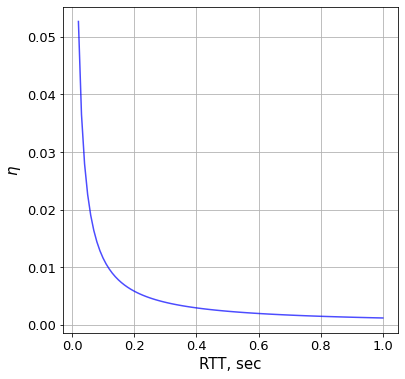
\includegraphics[width = 1\textwidth]{sw_rtt}}
		\end{figure}
	\end{center}
	\centering 
\end{column}
	\begin{column}{0.5\textwidth}  %%<--- here
		\begin{center}
			\begin{figure}[H]
				\center{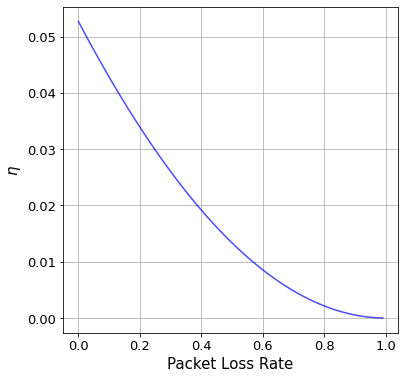
\includegraphics[width = 1\textwidth]{sw_plr}}
			\end{figure}
		\end{center}
		\centering 
	\end{column}
\end{columns}


\end{frame}